%%
%% licence       kaneton licence
%%
%% project       kaneton
%%
%% file          /home/mycure/kaneton/view/papers/assignments/k1.tex
%%
%% created       matthieu bucchianeri   [tue feb  7 11:49:38 2006]
%% updated       julien quintard   [sun feb 26 18:16:53 2006]
%%

%
% k1
%

\section{k1}

%
% overview
%

\subsection{Overview}

The \textbf{k1} project consists in the development of the bootloader.

In kaneton, one of the bootloader's role is to prepare a correct
execution context for the kernel.

To do so, the bootloader has to install the proper memory addressing model
the kernel is expecting, depending on the architecture. In fact, the
kaneton microkernel assumes it is running on a microprocessor architecture
with virtual memory enabled.

Therefore, the architecture dependent source code has to deal with that,
providing kind of virtual memory so the kaneton microkernel can be executed.

Let's take some examples; for the \textit{ia32-virtual} architecture,
the booloader will install the virtual memory using microprocessor's
facilities while for the \textit{ia32-segment} architecture, the booloader
and the entire architecture dependent source code will emulate this
virtual memory using microprocessor's segmentation facilities in a very
specific way.

Another bootloader's role is to provide the kernel enough information
on the current microprocessor's architecture.

To do so, the bootloader has to fill in an information structure which
will be passed to the kernel at its boot time.

This structure will inform the kernel of the location of some
fundamental objects like the kernel code, the kernel stack, the information
structure, the modules, the segments, the regions and the alloc survey area.

We will now detail some of these components:

\subsubsection{The Modules}

We call modules any additionnal file passed at the boot time.

A \textbf{module} can be a picture, a binary object, a configuration file
or anything else.

Do not consider a module in the other kernels terms. A kaneton module
can be anything while the term \textit{module} is generally used to describe
a kernel module, a dynamic part of code which can be attached to the
running kernel.

In kaneton, modules are used to pass the kaneton configuration file
which contains the kaneton parameters and describes the kaneton servers
to launch as soon as possible. The kaneton servers' binary objects to
launch are also passed as modules.

Of course the bootstrap has to handle kind of modules, otherwise it will
not be capable of passing them to the bootloader.

The bootloader must build a special data structure containing everything
necessary to get access to the modules including: number of modules,
modules' information, modules' contents etc..

In fact, the kernel itself will not use the modules. Indeed, a dedicated
server will be launched by the kernel and will get access to the modules.
Then this dedicated server will launch the very first servers and
parameterize the kernel.

To do so, the kernel will first launch this dedicated server and then
will explicitly give the area containing the modules to this dedicated
server.

It is obviously simpler to give one area containing the modules
stuff rather than giving an area containing the modules information, then
an area per module and finally another area containing the modules' string
names.

For these reasons, a very specific area must be built to contain
to whole stuff in relation with the modules so the kernel just has to
give this area to the dedicated server.

The modules area has the following form:

\begin{enumerate}
  \item
    A \textit{t\_modules} structure specifying some general information on
    the modules like the number of modules.
  \item
    An array of variable length modules, each module being composed of:

    \begin{enumerate}
      \item
	A descriptor \textit{t\_module} containing the module's size and
	a pointer to the module's name.
      \item
	The module contents.
      \item
	The module's string name terminated by a zero character.
    \end{enumerate}
\end{enumerate}

Be  careful;  the   array  of  modules  is  a   variable  length  item
array. Module data and name are variable length blocks.

The dedicated server will refer to the module descriptors to browse
throught the modules.

The calculation used to compute the next module address is:

\begin{verbatim}
sizeof(t_module) + module->size + strlen(module->name) + 1
\end{verbatim}

A smart idea would be to add a \textit{next} field in the \textit{t\_module}
structure to directly go through the next module.

\subsubsection{The Segments}

A \textbf{segment} is simply a contiguous area of used physical memory.

We introduced the term for nomenclature reasons.

Notice that a segment in the kaneton terms has nothing to do with
a segment in some architectures terms.

In fact, the kaneton kernel has to provide physical memory operations to
reserve, release, modify properties of the physical memory areas or segments.
To do so, the kaneton kernel is composed of a \textbf{segment manager} which
provide an interface to manipulate the segments.

As an example, let's consider the segment reservation which is a very
common segment operation. This operation looks for a contiguous area
of unused physical memory in its internal data structure and then
returns an identifier on this area.

Now consider that, at the kernel boot time, the segment manager has
an empty data structure. Then the segment manager can choose any
unused area and return an identifier on it. \textit{any unused area} means
any unused physical memory area including the kernel code area, the kernel
stack area, the modules area, the architecture dependent areas like maybe the
video memory area and the BIOS mapping area etc..

You should understand that the bootloader must build a data structure
containing the set of pre-reserved segments. By pre-reserved segments we
mean every fundamental and distinctive areas.

This data structure will be used by the task manager to properly
initialize the kernel address space used by the kernel task object.

Therefore it will be impossible, for example, to reserve an area
already hold for something else.

Notice that once the segment data structure has be used to initialize
the kernel's address space, its memory can be released.

\subsubsection{The Regions}

A \textbf{region} is a contiguous area of used virtual memory.

A region maps a segment part, or the whole.

You should have noticed that many fields of the initialization structure
are used to initialize parts of the kernel and then become useless.

Therefore, once the kernel is initialized, these fields and their memory
are no longer necessary.

So the segments and regions in relation with these fields can be released.

In fact, every time a kernel's manager will end its initialization; it will
release the needless memory reserved for this initialization.

For the regions, we decided to adopt another way rather than destroying
or resizing a region every time a segment or region becomes needless.

Indeed, the bootloader will so build a data structure describing the regions
once the kernel initialization is done.

The kernel's region manager will so go through this data structure and
rebuild the virtual memory from this data structure.

For the same reason than the segment data structure, the region data
structure should be released once the kernel's address space is
initialized.

\subsubsection{The Survey Area}


\newpage

\begin{verbatim}

XXX tous les kernels bootent d'une maniere crade car ils faut que le
XXX gestionnaire de memoire physique fournissent de la memoire. donc il
XXX doit avoir une structure de donnees pour savoir quelles zones sont
XXX libre ou utilisees. donc ce gestionnaire a besoin de memoire pour
XXX gerer sa structure de donner. rbef ca tourne en rond.

XXX generalement les gestionnaires de memoire physiques sont relativemtn
XXX laid car ils se gerent eux meme et donc font des tableaux statiques
XXX evolutifs via linkage par exemple.

XXX dans kaneton on voulait que tout le code du kernel soit propre.

XXX donc on voulait que toutes les structures de donnees soient gereees
XXX par le set manager qui lui meme se repose sur malloc().

XXX donc on a decider de fournir a malloc une zone de survie dans laquelle
XXX il peut gerer la memoire le temps que le boot du kernel ait passer
XXX l'etape du segment manager et du region manager. apres cela
XXX ca fonctionne car quand malloc() n aura plus de memoire il fera
XXX appel a segment_rsv() puis region_rsv()

\end{verbatim}

%
% assignments
%

\subsection{Assignments}

This  bootloader relocates  the  stuffs needed  by  the future  kernel
execution, allocate  a bunch of memory for  kernel initialization, and
provides to the kernel a complete initialization structure.

The relocation is not really necessary but we wanted the students
to understand low-level programming and more especially programming
in a very strict environment with no fine-grain allocator provided.

So in this project, the student has to write the entire code of the
bootloader. The only requirement is to be compliant with the structure
passed to the kernel.

Students also  have to write a  tiny console driver. Try  to make this
driver code generic so you can reuse it in the next steps.

The initialization structure called \textbf{t\_init} is defined in the
file \textit{core/include/kaneton/init.h}.

The \textbf{mem} and \textbf{memsz} fields indicate the available physical
memory of the system.

The \textbf{kcode} and \textbf{kcodesz} fields indicate the location and
size of the kernel binary in main memory after relocation.

The \textbf{init} and \textbf{initsz} fields indicate the location and
size of this init structure in main memory.

The \textbf{modules} and \textbf{modulessz} fields indicate the
location of the area used to store the modules.

The  \textbf{nsegments},   \textbf{segments}  and  \textbf{segmentssz}
fields indicate  the area location containing the  segment array. This
array describes the core's  pre-reserved segments. For the bootloader,
the  only required  fields of  the \textbf{o\_segment}  structures are
\textbf{segid}, \textbf{address}, \textbf{size} and  \textbf{perms}.
Other fields will be filled at kernel initialize time. Note that the
\textbf{segid} field must be equal to the \textbf{address} one.

The \textbf{nregions},  \textbf{regions} and \textbf{regionssz} fields
indicate  the area location  containing the  region array.  This array
describes the  segments to be  mapped after the initialisation  of the
core   region   manager.   You   must   fill   the   \textbf{address},
\textbf{offset} and \textbf{size} fields of each structure.

Indeed, many segments will be needless so this array only specify the
fundamental segments to map.

The \textbf{kstack} and \textbf{kstacksz} fields indicate the kernel
stack area location.

The \textbf{alloc}  and \textbf{allocsz} fields  indicate the location
and size  of the fine-grain allocator  survey area. This  area will be
used by  the \textbf{malloc()}  suite functions to  provide fine-grain
allocator  while no  segment  neither region  manager are  initialised
yet. You may allocate about 16 pages.

The  init  structure   also  contains  machine-dependent  fields,  the
\textbf{gdt} and the \textbf{page-directory}  if needed.  See the file
\textit{core/include/arch/[arch]/kaneton/init.h}  for  this  structure
(called \textbf{d\_init}).

The code provided must be located in the directory
\textit{core/bootloader/arch/[architecture]/}.

The students should use the system defines. Be aware that this project
must lead students to understand the project source organisation.

The student will have to build the init structure using the minimum
of memory, the goal of the game being to pack this structure.

Try to  think about a  very simple memory allocator  delivering single
pages or contiguous areas.

Assume that  the kernel is the  first given module.  Before jumping to
its  code,  you   must  switch  to  a  new   stack  reserved  for  the
kernel.  Remember that  switching system  stack in  a  single function
makes  impossible to  access previously  declared local  variables and
function arguments. So you will need global variables.

The kernel  should never return  after its call.  But as there  can be
loading  errors  or  code  errors,  you  must  suppose  that  it  will
return. In this case, you have to restore the old (bootloader's) stack
and display an error message.

Displaying  module  names, sizes  and  relocation  information is  the
minimum  requirement.   Having  an  enhanced display  of  pre-reserved
segments and regions will be very appreciated, but is not required.

%
% ia32
%

\subsection{IA-32 implementation}

The physical memory layout for the Intel architecture is the following:

\centerline{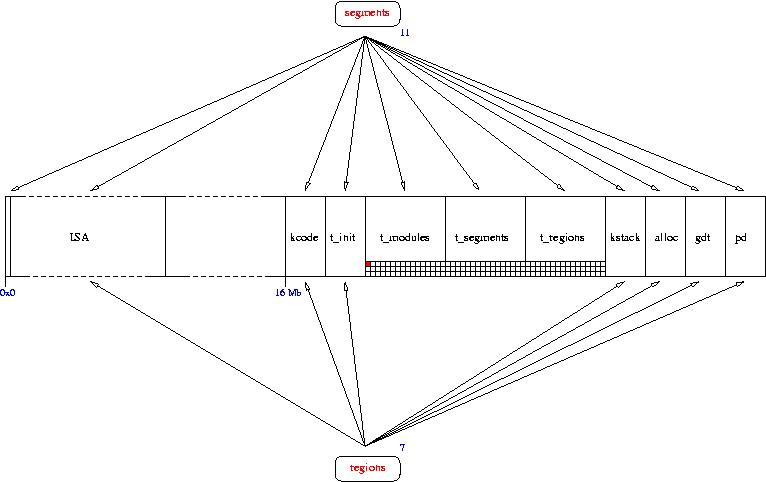
\includegraphics[scale=0.5]{figures/k1-memory-layout.jpg}}

All the segments must be mapped at the kernel boot time.

Notice that the  very first page \textbf{must not}  be mapped. Mapping
this page will cause null pointers to be valid !

Be careful to correctly initialise the machine-dependent fields
including \textbf{gdt} and \textbf{pd} which will be used by the microkernel
to retrieve the structures in main memory.

For this project,  you have to choose between using  paging or not. Be
careful:  once  this choice  done,  you  must  keep it  for  following
projects.

Here are the two possibilities:

\begin{itemize}
\item ia32-virtual, where you use paging
\item ia32-segment, without paging
\end{itemize}

---

Needless to  say, the  student will have  to install and  activate the
protected mode and the  virtual memory (students choosing ia32 without
paging will have to find an alternative to virtual memory).

Even if  the multi-bootloader  (GRUB for example)  activated protected
mode, you must ensure that it is correctly installed.

XXX lister les segments a mettre dans le tableau de segments et dire
XXX que le tableau de segment lui meme ne servira plus, enfin on peut
XXX le liberer une fois utilise, meme chose pour le tableau de regions
XXX qu on peut liberer completement une fois utilise

